\documentclass[tikz,border=8pt]{standalone}
% Shared look for every TikZ diagram. Load with % Shared look for every TikZ diagram. Load with % Shared look for every TikZ diagram. Load with \input{../../tools/tikz-style.tex}
\usepackage[T1]{fontenc}
\usepackage{lmodern}
\renewcommand{\sfdefault}{lmr}  % diagrams use the same serif as the text
\usetikzlibrary{arrows.meta, positioning, shapes.geometric, calc, fit, backgrounds}
\definecolor{cblue}{HTML}{4C78A8}
\definecolor{corange}{HTML}{F58518}
\definecolor{cgreen}{HTML}{54A24B}
\definecolor{cred}{HTML}{E45756}
\definecolor{cpurple}{HTML}{B279A2}
\definecolor{cgrey}{HTML}{6B6B6B}
\tikzset{
  every picture/.style={font=\sffamily, line width=1.2pt},
  box/.style={draw=#1, fill=#1!12, rounded corners=4pt, align=center, inner sep=7pt, minimum height=1.1cm},
  box/.default=cgrey,
  arrow/.style={-{Stealth[length=3mm]}, draw=cgrey, line width=1.4pt},
  title/.style={font=\sffamily\bfseries\Large},
  note/.style={font=\sffamily\small, text=cgrey, align=center},
}
\AtBeginDocument{\hyphenpenalty=10000 \exhyphenpenalty=10000}

\usepackage[T1]{fontenc}
\usepackage{lmodern}
\renewcommand{\sfdefault}{lmr}  % diagrams use the same serif as the text
\usetikzlibrary{arrows.meta, positioning, shapes.geometric, calc, fit, backgrounds}
\definecolor{cblue}{HTML}{4C78A8}
\definecolor{corange}{HTML}{F58518}
\definecolor{cgreen}{HTML}{54A24B}
\definecolor{cred}{HTML}{E45756}
\definecolor{cpurple}{HTML}{B279A2}
\definecolor{cgrey}{HTML}{6B6B6B}
\tikzset{
  every picture/.style={font=\sffamily, line width=1.2pt},
  box/.style={draw=#1, fill=#1!12, rounded corners=4pt, align=center, inner sep=7pt, minimum height=1.1cm},
  box/.default=cgrey,
  arrow/.style={-{Stealth[length=3mm]}, draw=cgrey, line width=1.4pt},
  title/.style={font=\sffamily\bfseries\Large},
  note/.style={font=\sffamily\small, text=cgrey, align=center},
}
\AtBeginDocument{\hyphenpenalty=10000 \exhyphenpenalty=10000}

\usepackage[T1]{fontenc}
\usepackage{lmodern}
\renewcommand{\sfdefault}{lmr}  % diagrams use the same serif as the text
\usetikzlibrary{arrows.meta, positioning, shapes.geometric, calc, fit, backgrounds}
\definecolor{cblue}{HTML}{4C78A8}
\definecolor{corange}{HTML}{F58518}
\definecolor{cgreen}{HTML}{54A24B}
\definecolor{cred}{HTML}{E45756}
\definecolor{cpurple}{HTML}{B279A2}
\definecolor{cgrey}{HTML}{6B6B6B}
\tikzset{
  every picture/.style={font=\sffamily, line width=1.2pt},
  box/.style={draw=#1, fill=#1!12, rounded corners=4pt, align=center, inner sep=7pt, minimum height=1.1cm},
  box/.default=cgrey,
  arrow/.style={-{Stealth[length=3mm]}, draw=cgrey, line width=1.4pt},
  title/.style={font=\sffamily\bfseries\Large},
  note/.style={font=\sffamily\small, text=cgrey, align=center},
}
\AtBeginDocument{\hyphenpenalty=10000 \exhyphenpenalty=10000}

\begin{document}
% Section 4: equal votes (bagging) against weighted votes (boosting). Bagging: answers 1, 1, 0, 1 with equal weight
% give 3 against 1. Boosting: answers 1, 1, 0 with alphas 0.8, 1.5 and 5 give 2.3 for class 1 against 5 for class 0.
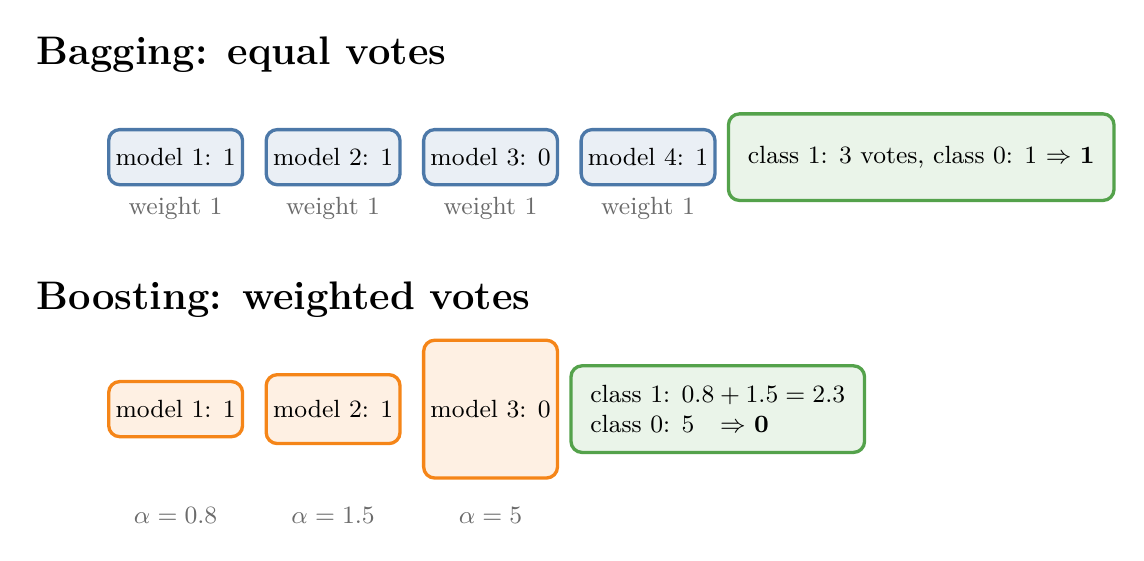
\begin{tikzpicture}[m/.style={box=#1, minimum width=1.7cm, minimum height=0.7cm, inner sep=2pt, font=\sffamily\small}]
  \node[title, anchor=west] at (-0.9, 1.3) {Bagging: equal votes};
  \foreach \a [count=\i] in {1,1,0,1} {
    \node[m=cblue] (b\i) at (2.0*\i - 1.0, 0) {model \i: \a};
    \node[note] at (2.0*\i - 1.0, -0.65) {weight 1};
  }
  \node[box=cgreen, font=\sffamily\small, anchor=west] at (8.0, 0) {class 1: 3 votes, class 0: 1 $\Rightarrow$ \textbf{1}};
  \node[title, anchor=west] at (-0.9, -1.8) {Boosting: weighted votes};
  \foreach \a/\w [count=\i] in {1/0.8, 1/1.5, 0/5} {
    \node[m=corange, minimum height=0.5cm + 0.25cm*\w] (o\i) at (2.0*\i - 1.0, -3.2) {model \i: \a};
    \node[note] at (2.0*\i - 1.0, -4.55) {$\alpha = \w$};
  }
  \node[box=cgreen, font=\sffamily\small, anchor=west, align=left] at (6.0, -3.2) {class 1: $0.8 + 1.5 = 2.3$\\class 0: $5$\quad$\Rightarrow$ \textbf{0}};
\end{tikzpicture}
\end{document}
